\PassOptionsToPackage{unicode=true}{hyperref} % options for packages loaded elsewhere
\PassOptionsToPackage{hyphens}{url}
%
\documentclass[]{article}
\usepackage{lmodern}
\usepackage{amssymb,amsmath}
\usepackage{ifxetex,ifluatex}
\usepackage{fixltx2e} % provides \textsubscript
\ifnum 0\ifxetex 1\fi\ifluatex 1\fi=0 % if pdftex
  \usepackage[T1]{fontenc}
  \usepackage[utf8]{inputenc}
  \usepackage{textcomp} % provides euro and other symbols
\else % if luatex or xelatex
  \usepackage{unicode-math}
  \defaultfontfeatures{Ligatures=TeX,Scale=MatchLowercase}
\fi
% use upquote if available, for straight quotes in verbatim environments
\IfFileExists{upquote.sty}{\usepackage{upquote}}{}
% use microtype if available
\IfFileExists{microtype.sty}{%
\usepackage[]{microtype}
\UseMicrotypeSet[protrusion]{basicmath} % disable protrusion for tt fonts
}{}
\IfFileExists{parskip.sty}{%
\usepackage{parskip}
}{% else
\setlength{\parindent}{0pt}
\setlength{\parskip}{6pt plus 2pt minus 1pt}
}
\usepackage{hyperref}
\hypersetup{
            pdftitle={Presence and Artificial Intelligence (PAI) Lab},
            pdfborder={0 0 0},
            breaklinks=true}
\urlstyle{same}  % don't use monospace font for urls
\usepackage[margin=1in]{geometry}
\usepackage{graphicx,grffile}
\makeatletter
\def\maxwidth{\ifdim\Gin@nat@width>\linewidth\linewidth\else\Gin@nat@width\fi}
\def\maxheight{\ifdim\Gin@nat@height>\textheight\textheight\else\Gin@nat@height\fi}
\makeatother
% Scale images if necessary, so that they will not overflow the page
% margins by default, and it is still possible to overwrite the defaults
% using explicit options in \includegraphics[width, height, ...]{}
\setkeys{Gin}{width=\maxwidth,height=\maxheight,keepaspectratio}
\setlength{\emergencystretch}{3em}  % prevent overfull lines
\providecommand{\tightlist}{%
  \setlength{\itemsep}{0pt}\setlength{\parskip}{0pt}}
\setcounter{secnumdepth}{0}
% Redefines (sub)paragraphs to behave more like sections
\ifx\paragraph\undefined\else
\let\oldparagraph\paragraph
\renewcommand{\paragraph}[1]{\oldparagraph{#1}\mbox{}}
\fi
\ifx\subparagraph\undefined\else
\let\oldsubparagraph\subparagraph
\renewcommand{\subparagraph}[1]{\oldsubparagraph{#1}\mbox{}}
\fi

% set default figure placement to htbp
\makeatletter
\def\fps@figure{htbp}
\makeatother


\title{Presence and Artificial Intelligence (PAI) Lab}
\author{}
\date{\vspace{-2.5em}}

\begin{document}
\maketitle

~

Inspired and guided by a Blue Sky workshop at the 2023 annual conference
of the International Communication Association, where I had the
opportunity to moderate a panel on which esteemed scholars like
\href{https://wmich.edu/communication/directory/edwards}{Autumn
Edwards}, \href{https://grady.uga.edu/faculty/sun-joo-grace-ahn/}{Sun
Joo (Grace) Ahn},
\href{https://dot.egr.uh.edu/departments/ilt/people/faculty/liao-tony}{Tony
Liao}, \href{https://drtammylin.com/}{Jih-Hsuan Tammy Lin}, and
\href{https://klein.temple.edu/directory/matthew-lombard-lombard}{Matthew
Lombard} shared their invaluable experience of founding and managing
research groups and spaces, I began to develop the Presence and
Artificial Intelligence (PAI) Lab in July 2023. Echoing the
pronunciation and significance of ``\textbf{\emph{π}}'', the PAI Lab
stands for its commitment to exploring infinite possibilities for
non-recurring emerging technology research.

This PAI Lab aims at conducting research on users' relationships with a
range of presence-evoking technologies, including social robots, virtual
humans, chatbots, virtual influencers, smartwatches, memes, virtual
reality, and augmented reality. The lab also delves into topics such as
explainable AI (XAI), Science and Technology Studies (STS), and
ubiquitous computing.

Revolving around both the science and the methods of artificial
intelligence, our lab seeks to conduct theoretically robust and
methodologically innovative research, with the support of the
technologies available in the lab space, including:\\
\emph{Aldebaran Robot NAO}\\
\emph{Double II Telepresence robot}\\
\emph{Meta Quest Pro}\\
\emph{UBTech Robot Alpha}\\
\emph{Robot Eilik}\\
\emph{Shimmer3 GSR+ Unit}\\
~\\
~\\
Graduate students at the PAI Lab combine technology research with a
variety of topics and contexts, including popular culture,
globalization, public health, semiotics, and big data. Our lab members
are:

\href{https://www.fanjueliu.com/}{Fanjue Liu} (graduated Fall 2024)

\includegraphics{images/fanjue.JPG}

~

Fanjue Liu was a doctoral student at the University of Florida. Her
research investigates how people perceive and interact socially with
emerging technologies such as virtual humans. Specifically, she
investigates how people use different psychological patterns to interact
with virtual influencers, how the emergence of virtual influencers
changes the dynamics of influencer marketing, and whether virtual
influencers can be considered a viable substitute for human
influencers.\\

\href{https://www.linkedin.com/in/xiaobei-chen/}{Xiaobei Chen}

\includegraphics{images/xiaobei.JPG}

~

Xiaobei Chen is a current PhD/MPH student with concentrations in health
communication and epidemiology. Her research areas include (1) using
emerging technologies as interventions for health professionals and
patients, (2) examining the association between health technologies and
disparities, and (3) exploring public health emergency communication on
social media. In terms of the topics, she focuses on cancer, infectious
diseases, and empathic communication in healthcare.\\

\href{https://www.jou.ufl.edu/staff/jiayue-lynn-li/}{Lynn Li}

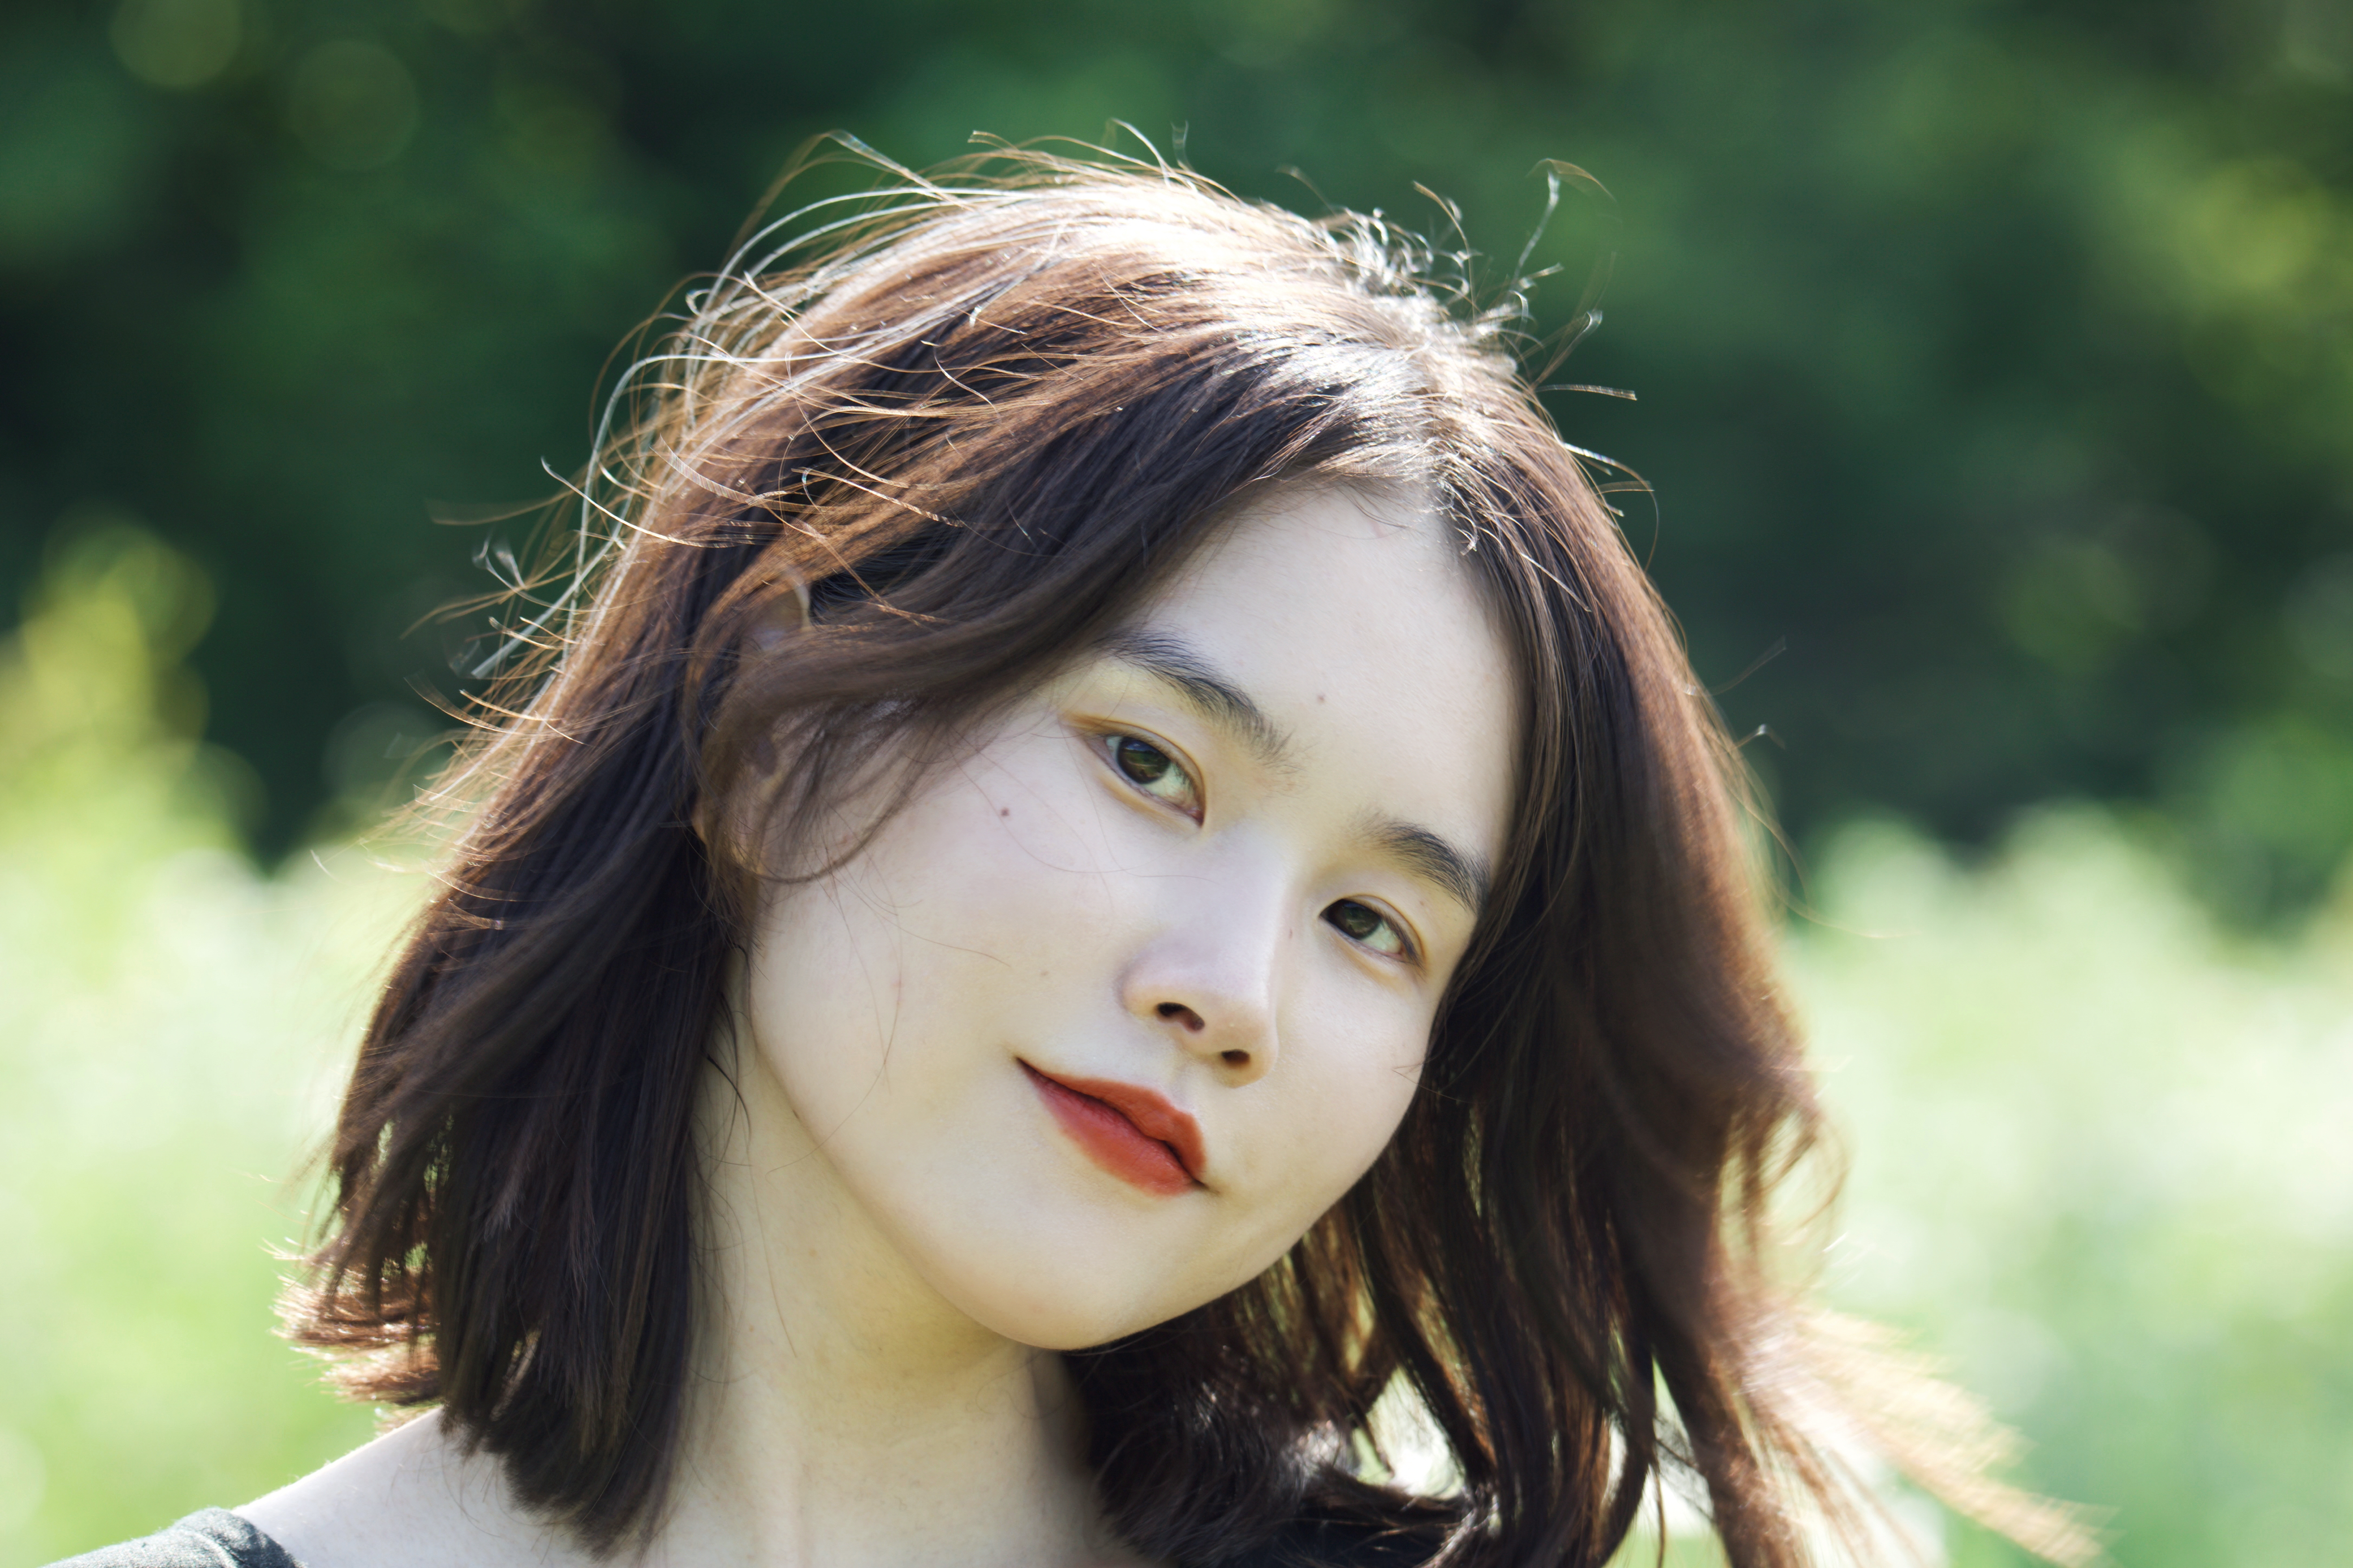
\includegraphics{images/jiayue.JPG}

~

Jiayue Lynn Li is a PhD student with a background in media, cultural,
and communication studies. Her research interests span digital
communication, human-computer/robot interaction, and critical media
analysis from a phenomenological standpoint. Her current projects focus
on how individuals interact with and make meanings from digital
artifacts such as memes created by selfies and (dis)embodied robots, and
how this shapes our understanding of the self, others, and the world.\\

\href{https://www.linkedin.com/in/yunxiao-caitlyn-chen-133413178/}{Yunxiao
Chen (Caitlyn)} (graduated December, 2023; currently Ph.D.~student at
Boston University)

\includegraphics{images/yunxiao.jpg}

~

Yunxiao Chen (Caitlyn) was a Master's student and a teaching \& research
assistant at the College of Journalism and Communications, UF. She
defended her thesis in October 2023. She is determined to being a
Human-Computer Interaction scholar and user experience expert (design +
research). Her future studies will broadly address the intersections of
people, information, and technology. Currently, she is researching human
attitudes and behaviors with emerging technologies, such as virtual
reality and smartwatches. With a background in language and literature,
Yunxiao is passionate about creative writing and has published some
poems, short stories, and translations in China. As a ``Cyberpunk''
enthusiast, she aspires to do various art stuff on this theme. She will
join the doctoral program in Emerging Media Studies at Boston
University.\\

\href{https://www.linkedin.com/in/loren-ruffin/}{Loren Ruffin}
(graduated May, 2023)

\includegraphics{images/LorenRuffin_CJCHeadshot.jpg} ~

Loren Ruffin was a Professional Master's student in the CJC and
completed an M.A.~in Mass Communication. Prior to attending UF, she
received a B.S. in Communication, with a concentration in Journalism,
from East Carolina University. Her study interests included
human-machine communication, digital user experiences, and diversity,
equity, and inclusion in digital products. As part of her capstone
project, she designed and programmed a virtual reality vocabulary game
focused on accessibility specifically for deaf and hard-of-hearing
users. Post-graduation she is currently a content designer for Uber's
Safety UX team, helping to design experiences that aim to keep earners
and consumers safe on the app.\\

\end{document}
